\documentclass{article}
\usepackage{url,apacite,graphicx}
\title{Multidimensional scaling of varietal data in sedimentary provenance analysis}
\author{P. Vermeesch\\\emph{University College London, United Kingdom}\\\\
  A. G. Lipp\\\emph{Merton College, University of Oxford, United Kingdom}\\\\
  D. Hatzenb\"{u}hler and L. Caracciolo\\\emph{FAU Erlangen-N\"{u}rnberg, Germany}\\\\
  D. Chew\\\emph{Trinity College Dublin, Ireland}
}
\date{}
\begin{document}

\maketitle

\begin{abstract}
Varietal studies of sedimentary provenance use the properties of
individual minerals or mineral groups. These are recorded as lists of
numerical tables that can be difficult to interpret. Multidimensional
Scaling (MDS) is a popular multivariate ordination technique for
analysing other types of provenance data based on, for example,
detrital geochronology or petrography.  Applying MDS to varietal data
would allow them to be treated on an equal footing with those other
provenance proxies. MDS requires a method to quantify the
dissimilarity between two samples. This paper introduces three ways to
do so. The first method (`treatment-by-row') turns lists of
(compositional) data tables into lists of vectors, using principal
component analysis. These lists of vectors can then be treated as
`distributional' data, and subjected to MDS analysis using
dissimilarity measures such as the Kolmogorov-Smirnov statistic.  The
second method (`treatment-by-column') turns lists of compositional
data tables into multiple lists of vectors, each representing a single
component of the varietal data. These multiple distributional datasets
are subsequently subjected to Procrustes analysis or 3-way MDS. The
third method uses the Wasserstein-2 distance to jointly compare the
rows and columns of varietal data. This arguably makes the best use of
the data but acts more like a `black box' than the other two
methods. Applying the three methods to a detrital titanite dataset
from Colombia yields similar results. After converting varietal data
to dissimilarity matrices, they can be combined with other types of
provenance data, again using Procrustes analysis or 3-way MDS.
\end{abstract}

\section{Introduction}\label{sec:intro}

Multidimensional Scaling \citeA<MDS>[]{kruskal1978, shepard1980,
  vermeesch2013} is a multivariate ordination technique that has
gained considerable popularity in recent years as a method to
interpret large datasets in sedimentary provenance analysis
\cite{vermeesch2013}. Given a table of pairwise `dissimilarities'
between samples, MDS produces a lower (typically two-) dimensional
`map' in which samples plot close together and dissimilar samples plot
far apart. MDS can be applied to a wide variety of different
provenance proxies by choosing an appropriate dissimilarity measure.
\citeA{vermeesch2019a} distinguishes between three different types of
provenance data, each of which is associated with a specific database
format (Figure~\ref{fig:datastructures}):

\begin{enumerate}
\item{\bf Distributional data} such as detrital zircon U-Pb ages can
  be stored in \textbf{lists of decimal numbers}, where each list
  represents a sample and typically contains a different number of
  values (i.e. single grain ages). Two samples can be compared using
  the Kolmogorov-Smirnov distance or related non-parametric statistics
  \cite{vermeesch2018b}. The resulting dissimilarity matrix fulfils
  the metric requirements and is therefore suitable for both classical
  and nonmetric MDS \cite{vermeesch2013}.
\item{\bf Compositional data} such as the major and trace element
  compositions of bulk samples are stored in \textbf{tables of decimal
    numbers}, in which the rows represent samples and the columns
  represent components such as elements or isotopes. Pairwise
  comparison of the samples (rows) is best done using the Aitchison
  distance, which corresponds to a Euclidean distance of centred
  logratios \cite{aitchison1986}. It can be shown that, in this case,
  (classical) MDS is mathematically equivalent to Principal Component
  Analysis \citeA<PCA>[]{aitchison1983, vermeesch2013}. The advantage
  of PCA over plain MDS is that it provides two sets of coordinates:
  one representing the rows and one representing the columns of the
  input data. This feature will be used in Section~\ref{sec:method2}
  of this paper.
\item{\bf Count data} such as the petrography or heavy mineral
  composition of sediment are stored in \textbf{tables of integers},
  in which rows correspond to samples, and columns to lithologies or
  minerals.  Pairwise comparison of samples of count data can be done
  using the Chi-square distance, which can handle zero values, unlike
  the Aitchison distance \cite{vermeesch2018d}. It can be shown that
  MDS of Chi-square distance tables is equivalent to Correspondence
  Analysis \cite[CA,]{greenacre1984}. Like PCA, CA also yields
  coordinates for the row and columns of the data tables, but these
  will not be discussed further here.
\end{enumerate}

This paper adds a fourth class of data to this list:

\begin{enumerate}
  \setcounter{enumi}{3}
\item{\bf Varietal data} capture the variations in optical or chemical
  properties shown by an individual mineral or mineral group
  \cite{morton1985b,morton1991}. This paper will focus on chemical
  properties, as measured by microanalytical techniques such as
  electron, laser or ion microprobe analysis. These data can be stored
  in \textbf{lists of compositional data tables}. Each table in a
  varietal dataset contains the same number of columns (representing
  elements or isotopes) and a different number of rows (representing
  individual analyses in a sample).
\end{enumerate}

Unlike distributional, compositional and count data, varietal data
have hitherto not been associated with a `natural' dissimilarity
measure. It is therefore not clear how varietal data can be analysed
by MDS. This is unfortunate, because the complex structure of varietal
data makes the need for multivariate ordination all the more
pressing. This paper addresses this issue, by proposing three
mechanisms to compare varietal data (Sections~\ref{sec:method1},
\ref{sec:method2} and \ref{sec:method3}). With these mechanisms in
place, varietal data can be treated on an equal footing with other
types of provenance data. Section~\ref{sec:3way} shows how varietal
data can be combined with distributional, compositional and count data
using 3-way MDS and Procrustes analysis.\medskip

The methods discussed in this paper are illustrated with a dataset
from Colombia's Sierra Nevada de Santa Marta (SNSM). This dataset
comprises 17~samples of modern river sediment, characterised by
12~different provenance proxies, including three distributional
datasets (detrital zircon, apatite and titanite U-Pb ages); four
compositional datasets (major and trace element composition of the
sand and clay fraction); two datasets of counts (petrography and heavy
minerals); and three varietal datasets (trace element compositions of
detrtial zircon, apatite and titanite). The geological details of the
dataset are not relevant to the present discussion and are only
briefly mentioned in this paper. The reader is referred to a separate
paper for further details \cite{caracciolo2023}.

\begin{figure}
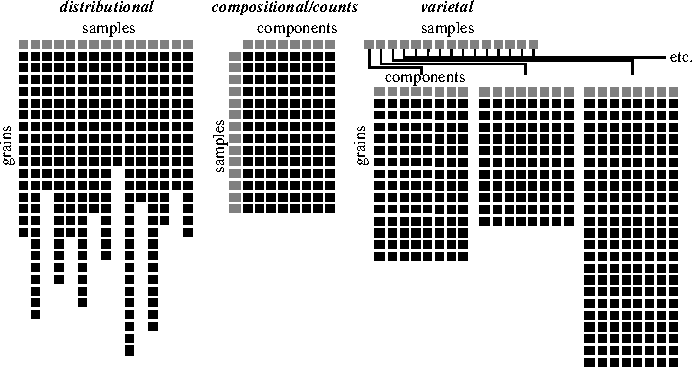
\includegraphics[width=\linewidth]{Fig1.pdf}
\caption{Schematic representation of the four classes of
  provenance data. Grey boxes represent labels and black boxes
  numbers. distributional data can be stored as lists of vectors,
  compositional data as tables of positive decimal numbers, count data
  as tables of non-negative integers, and varietal data as lists of
  tables with positive decimal numbers.}
\label{fig:datastructures}
\end{figure}

\section{Method~1: treatment by row}\label{sec:method1}

As explained in Section~\ref{sec:intro}, varietal data are, in
essence, lists of compositional data tables. Compositional data can be
compared using the Aitchison distance, and subjected to PCA.  The
dimension-reducing properties of PCA can be used to turn a varietal
dataset into a distributional dataset:

\begin{enumerate}
\item Pool all the samples together to create one large compositional
  dataset, i.e. a single table in which each row represents an
  analysis, and each column represents an element or isotope.
\item Subject this data table to PCA. Return the first principal
  component, which accounts for the largest proportion of the overall
  variance, and discard the other principal components.
\item Parse the first principal component vector into different
  samples. This results in a list of vectors or, in other words, a
  distributional dataset. This can then be analysed by MDS with the
  usual Kolmogorov-Smirnov statistic.
\end{enumerate}

Figure~\ref{fig:method1} applies the treatment-by-row strategy to the
titanite chemistry data from the SNSM. Figure~\ref{fig:method1}.a
shows the first two principal components of the pooled titanite
compositions on a biplot. Only the first of these components (PC1) is
used for subsequent distributional analysis. It is dominated by Pb,
Fe, W, Sr and Al, which are assocated with negative loadings (red
arrows in Figure~\ref{fig:method1}.a), and the light lanthanides (La,
Ce, Pr, Nd) and actinides (U, Th), which are assocated with positive
loadings. PC1 accounts for 51\% of the total variance among the 25
components. This means that 49\% of the variance is discarded,
including the 19\% that is associated with PC2. It is the necessary
sacrifice that is needed to turn the varietal dataset into a
distributional one.\medskip

The distributions of PC1 are shown as kernel density estimates (KDEs)
in Figure~\ref{fig:method1}.b. It is the shapes of these distributions
that are used as a secondary provenance proxy. Inspecting the KDEs by
eye shows some clear groupings. Samples TAP, MAR, RAN and AGI are all
characterised by sharp unimodal PC1 distributions that are dominated
by positive values, which suggest that these samples are enriched in
rare earth elements relative to Pb, Fe, W and Al. In contrast, samples
such as SEV, GUC, COR and FRI are characterised by broader PC1
distributions that are shifted towards more negative values. This
suggests that these samples are enriched in Pb, Fe, W and Al relative
to the rare earths, in comparison with samples SEV, GUC, COR and
FRI.\medskip

A more objective comparison of the PC1 distributions is achieved by
MDS analysis, using the KS-statistic (Figure~\ref{fig:method1}.c).  As
expected, samples SEV, GUC, COR and FRI cluster closely together on
the MDS map, opposite to samples MAR, TAP, AGI and RAN. This grouping
makes geological sense, as SEV, GUC, COR and FRI were collected from
river catchments that drain metamorphic lithologies (migmatite,
gneiss, metadiorite), whereas samples MAR, TAP, AGI and RAN were
collected from catchments that drain igneous lithologies
\cite{caracciolo2023}.

\begin{figure}
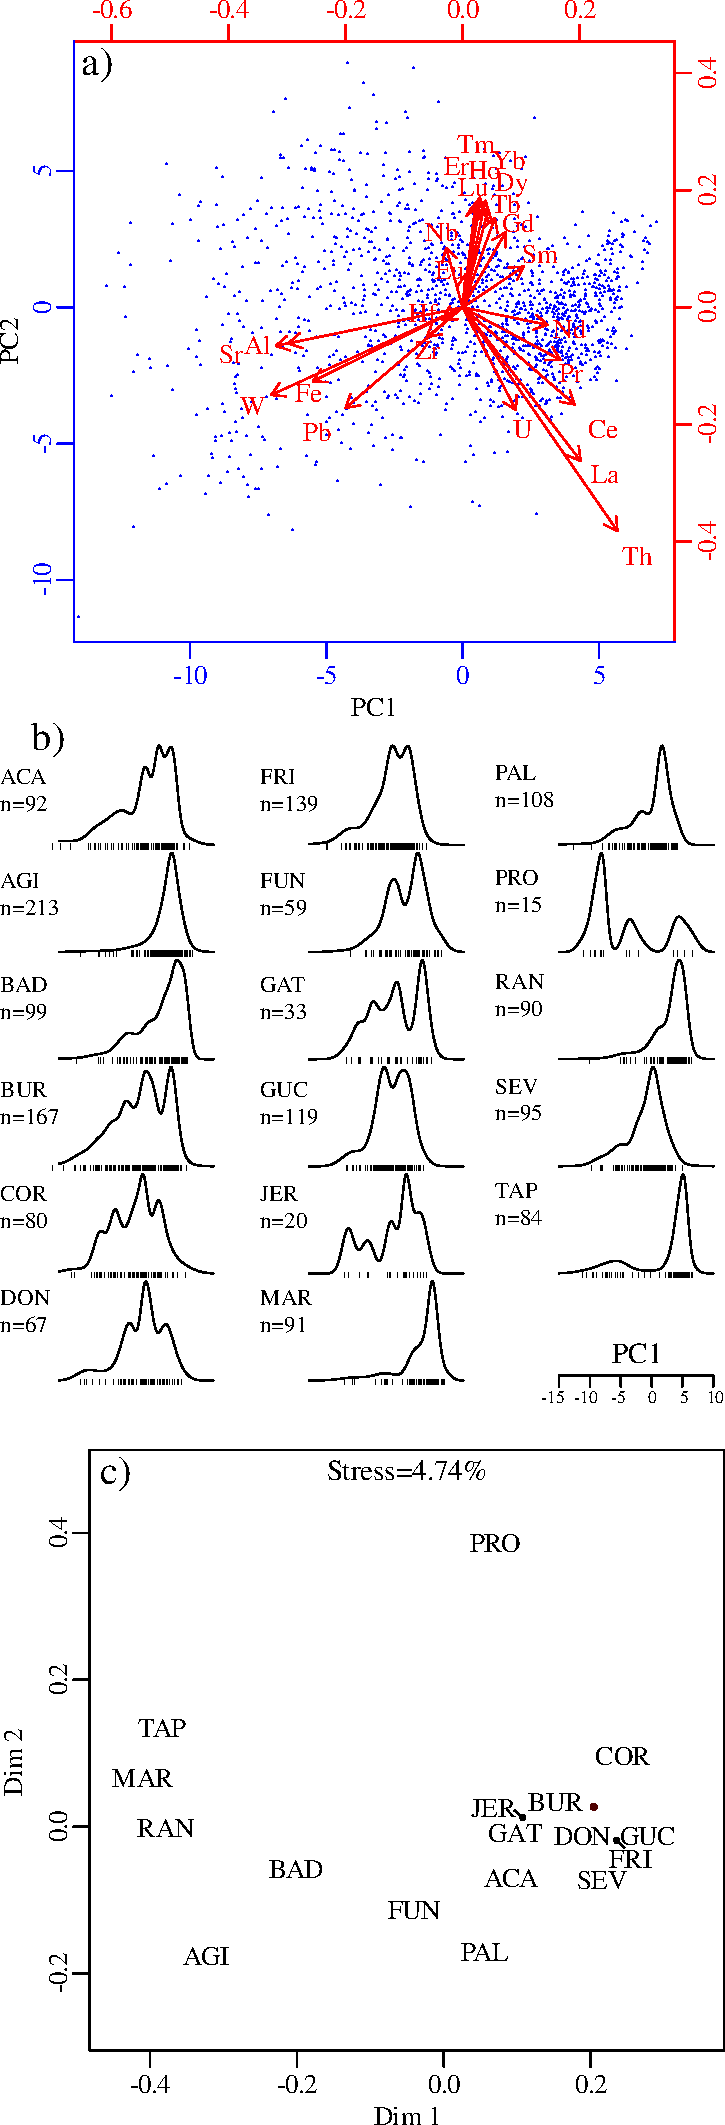
\includegraphics[height=.7\textheight]{Fig2.pdf}
\caption{a) PCA biplot of the pooled titanite geochemistry data. The
  blue dots mark 1,571 titanite analyses, which belong to 17
  samples. b) Kernel density estimates (bandwidth = 0.8) of the first
  principal component (PC1) of the 17 samples; c) Nonmetric MDS
  configuration of the 17 PC1 distributions, using the
  Komogorov-Smirnov statistic as a dissimilarity measure. MDS
  coordinates are located in the middle of the plot labels. The
  Kruskal Stress value suggests a `good' fit.}
\label{fig:method1}
\end{figure}

\section{Method~2: treatment by column}\label{sec:method2}

The treatment-by-row approach turns the varietal data into a single
distributional dataset. An alternative approach is to turn it into
multiple distributional datasets:

\begin{enumerate}
\item Break the compositional data table of each sample up into its
  components (columns), and treat each of these components as a
  distributional dataset. In other words, a varietal dataset
  comprising $n$ samples and $m$ components (e.g., elements), can be
  turned into $m$ distributional datasets containing $n$ samples (each
  in turn containing a variable number of analyses).
\item Compute the dissimilarity matrices of all the distributional
  datasets and stack them together to form a multidimensional array of
  size ${n}\times{m}\times{m}$.
\item Subject the stack of dissimilarity matrices to Procrustes
  analysis or 3-way MDS \cite{carroll1970, gower1975,
    vermeesch2015}. For Procrustes analysis, this produces a similar
  set of coordinates as Method~1.  For 3-way MDS, it produces two sets
  of coordinates: one for the rows (samples) and one of the columns
  (components). In this respect, 3-way MDS is somewhat similar to PCA.
\end{enumerate}

Applying the treatment-by-column approach to the SNSM data,
Figure~\ref{fig:method2}.a shows the output of a Generalised
Procrustes Analysis \citeA<GPA>[]{gower1975}. It uses affine
transformations to obtain a single set of coordinates from the 25
compositional MDS configurations. The results in
Figure~\ref{fig:method2}.a look remarkably similar to the MDS
configuration of Figure~\ref{fig:method1}.c, despite the completely
different mechanism behind it. In both case, samples SEV, GUC, COR and
FRI cluster closely together, in an opposite corner from samples MAR,
TAP, AGI and RAN. The only major difference between the MDS
(Figure~\ref{fig:method1}.c) and GPA (Figure~\ref{fig:method2}.a)
configurations is the 45 degree clockwise rotation of the latter with
respect to the former. This is expected since GPA is rotation
invariant.\medskip

One limitation of GPA is the fact that all compositional information
is lost in the visualisation. This issue is addressed by 3-way MDS, as
shown in Figures~\ref{fig:method2}.b and c. Together, these two pieces
of graphical output display both the row names and the column names of
the varietal dataset. The `group configuration' of the samples
(Figure~\ref{fig:method2}.b) is similar to the output of the GPA and
(2-way) MDS configurations of Figures~\ref{fig:method1}.c and
\ref{fig:method2}.a: once again, samples SEV, GUC, COR and FRI plot
separately from samples MAR, TAP, AGI and RAN. However, the 3-way MDS
configuration (Figure~\ref{fig:method2}.b) is less similar to the GPA
configuration (Figure~\ref{fig:method2}.a) than the GPA configuration
is to the 2-way MDS analysis (Figure~\ref{fig:method1}.c).\medskip

The great appeal of 3-way MDS lies in the combination of the group
configuration with the source weights, which are shown in
Figure~\ref{fig:method2}.c. These weights show the relative importance
that the two dimensions of the group configuration attach to the 25
compositional variables.  Pb, Fe, W and Al plot at the upper left end
of the subject weights. They are associated with light horizontal
weights (x-coordinates of 0.7--0.8) and heavy vertical weights
(y-coordinates of 1.7--2.0).  The rare earth elements (except Eu) plot
at the opposite end of the subject weights, and are associated with
comparatively heavy horizontal weights (x-coordinates of 1.0--1.1) and
light vertical weights (y-coordinates of 0.7--1.0). Note that the
grouping of the elements is in good agreement with the loadings of the
first principal component (Figure~\ref{fig:method1}.a).\medskip

The weights tells us that the horizontal dimension (Dim 1) of the
group configuration (Figure~\ref{fig:method2}.b) is controlled by
variability in the rare earth composition, whereas the vertical
direction (Dim 2) is controlled by variability in the Pb, Fe, W and Al
concentrations.

\begin{figure}
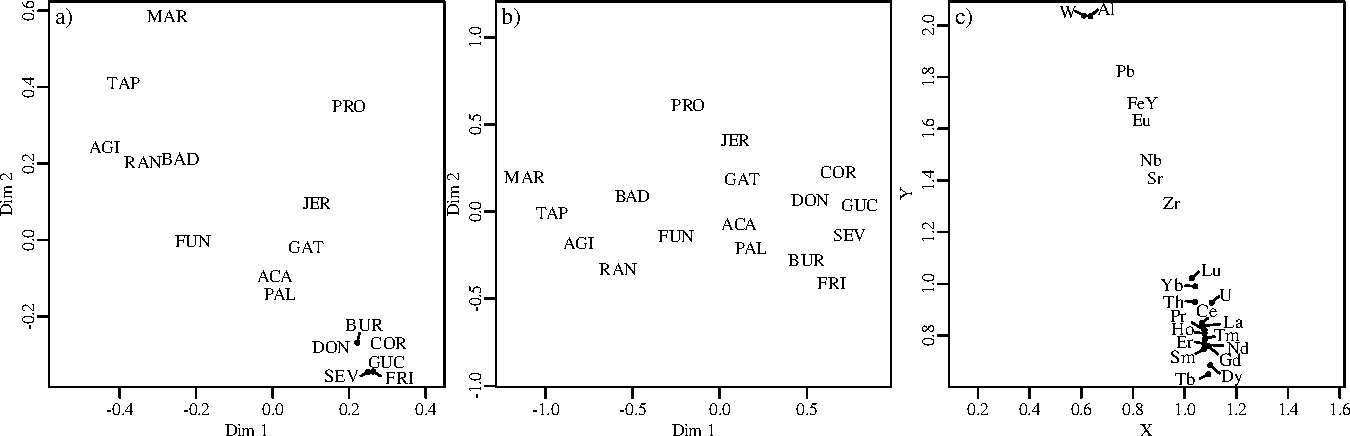
\includegraphics[height=.7\textheight]{Fig3.pdf}
\caption{a) Procrustes analysis of the 25 MDS configurations that are
  obtained by breaking the titanite chemistry data up into 25
  distributional datasets; b) Group configuration of a 3-way MDS
  analysis of the 25 dissimilarity matrices extracted from the same
  titanite geochemistry dataset; c) Source weights of the 3-way MDS
  analysis, showing the stretching factors that are associated with
  each of the 25 components. These can be combined with the group
  configuration to yield 25 `private spaces' \protect\cite{arabie1987,vermeesch2015}.}
\label{fig:method2}
\end{figure}

\section{Method~3: Wasserstein-2 distance}\label{sec:method3}

Thus far we have seen how varietal data can be turned into
distributional data, either by treating the compositions of each
sample by row (method~1, Section~\ref{sec:method1}) or by column
(method~2, Section~\ref{sec:method2}). In this Section, rows and
columns will be treated jointly, using the principles of optimal
transport (OT). OT is a burgeoning field of mathematics that is
concerned with the constrained allocation of limited resources to
achieve the greatest effect.\medskip

The `Wasserstein-p' distance ($W_p$) is a key concept in the field of
OT. A classical metaphor for the $W_p$-distance is the minimum amount
of work that needs to be done to transform a pile of earth into a
different pile of earth with the same volume but different location
and shape. Based on this analogy, the $W_p$-distance is also known as
the ``earth mover's distance''. Distributional data can be treated as
1-dimensional `piles of earth'. In this case, the $W_1$-distance
between two samples simply equates to the area between their
respective empirical cumulative distribution functions (ECDFs):

\begin{equation}
  W_p(A,B) = \left(\int\limits_{0}^{1}
  \left|F_A^{-1}(x)-F_B^{-1}(x)\right|^p dx
  \right)^{\frac{1}{p}}
  \label{eq:Wp}
\end{equation}

\noindent where $A$ and $B$ are two distributional datasets, $F_A$ and
$F_B$ are their respective ECDFs, and $F_A^{-1}$ and $F_B^{-1}$ are
the corresponding quantile functions. The $W_2$-distance is slightly
less intuitive than the $W_1$-distance but is nevertheless preferred
because it mathematically behaves like a Euclidean distance. The $W_1$
and $W_2$ distances fulfil the metric requirements and can therefore
be subjected to both classical and metric MDS.\medskip

\citeA{lipp2022} show that the $W_2$-distance produces results that
are often equivalent and sometimes better than those obtained by the
KS-statistic.  Thus, we could substitute the KS-statistic for the
$W_2$-distance in Sections~\ref{sec:method1} and
\ref{sec:method2}. Alternatively, it is also possible to apply the
$W_2$-distance directly to the varietal data, without conversion to
distributional data, by generalising Equation~\ref{eq:Wp} from one to
two dimensions:

\begin{equation}
  W_p(A,B) = \left(
  \min\limits_{\pi\in\Pi}\int c(x,y)^p d\pi(x,y)
  \right)^{\frac{1}{p}}  
  \label{eq:Wp2D}
\end{equation}

\noindent where $\pi$ is the `transport plan', i.e. a probability
distribution in which $d\pi(x,y)$ is the amount of material that is
transported from location $x$ to $y$; and $c(x,y)$ is the `cost'
associated with this transport. Given two compositional tables ($X_A$
and $X_B$, say) of size ${n_A}\times{m}$ and ${n_B}\times{m}$,
respectively the `cost matrix' is obtained by computing the Aitchison
distance between each row of table $X_A$ and each row of table
$X_B$. This results in a matrix of size ${n_A}\times{n_B}$. The
optimal transport plan is obtained from this cost matrix by linear
programming \cite{villani2021}, the principles of which go beyond the
scope of this paper.\medskip

Computing the $W_2$-distance to all sample pairs in a varietal dataset
yields a square dissimilarity matrix that can be analysed by MDS.  For
the SNSM titanite dataset, this yields a configuration that looks
broadly similar to the results obtained by methods~1 and 2
(Figure~\ref{fig:method3}). Notable exceptions are samples PRO and
JER, which are significantly further removed from the bulk of the
dataset than they are in Figures~\ref{fig:method1}.c,
\ref{fig:method2}.a and \ref{fig:method2}.b. This behaviour is likely
a consequence of the small number of analyses in these two samples (20
for JER and 15 for PRO, see Figure~\ref{fig:method1}.b), as confirmed
by the uncertainty regions of Figure~\ref{fig:method3}.b, which
correspond to the convex hull of 20 bootstrapped replicates for each
sample. Repeating the same procedure for method~1 produces uncertainty
regions that are, on average, larger than for method~3, but more
uniform in size. This suggests that the `treatment-by-row' approach is
less precise than the Wasserstein approach, but also less
`heteroscedastic'. \medskip

The advantage of method~3 over the other two methods is that it makes
full use of the entire dataset, including any covariance structure
that may be embedded therein. The disadvantage is that the
compositional information is lost in the process of calculating the
cost matrix. Therefore, method~3 acts more like a `black box' than
method~1 and certainly more than method~2.\medskip

\begin{figure}
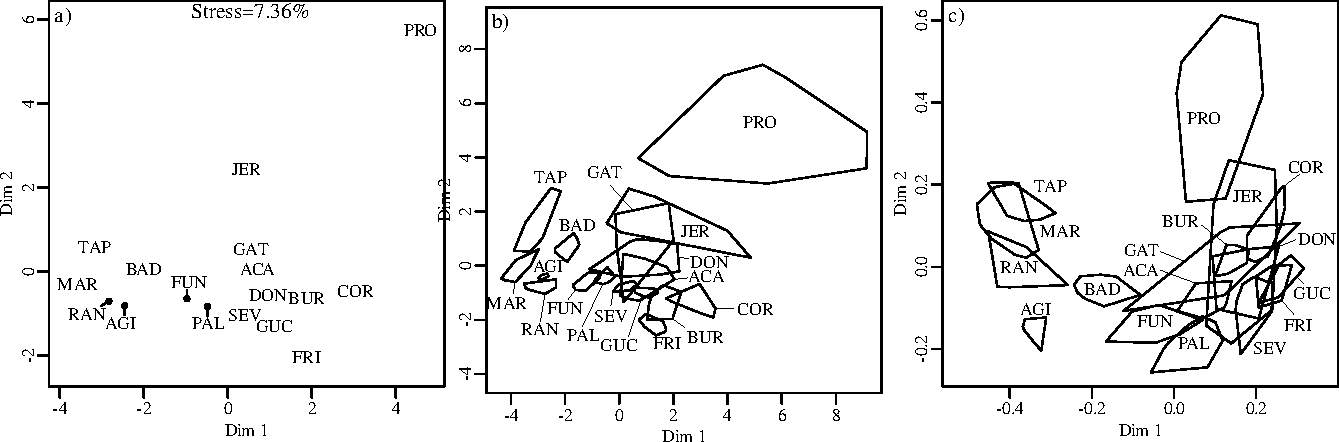
\includegraphics[height=.7\textheight]{Fig4.pdf}
\caption{a) Nonmetric MDS configuration of the titanite data using the
  Wasserstein-2 distance (method~3). Although the Kruskal Stress value
  is higher than for Figure~\ref{fig:method1}.a, this does not
  necessarily mean that the configuration is less informative than
  that of method~1. The higher stress values just means that it was
  more difficult for the MDS algorithm to fit the dissimilarity matrix
  to a 2-dimensional configuration of points.  The fit still qualifies
  as `good'. b) Uncertainty regions of the MDS configuration, obtained
  by constructing the convex hull of 20 bootstrapped replicates of
  each sample. c) Bootstrapped uncertainty regions for the
  treatment-by-row results of Figure~\ref{fig:method1}.c.}
\label{fig:method3}
\end{figure}

\section{Combining varietal data with other provenance proxies}\label{sec:3way}

Section~\ref{sec:method2} showed how Procrustes analysis and 3-way MDS
can be used to combine multiple dissimilarity matrices together, and
extract a single configuration of samples from them. The same
techniques can also be used to combine varietal data with other
provenance proxies.  In principle, this can be done using any of the
three methods. However, in practice, methods~1 and 3 are the most
sensible choices, for the following reason.\medskip

There are 12 provenance proxies in the SNSM dataset, including three
varietal datasets, where the titanite, apatite and zircon compositions
comprise 25, 22 and 8 compositional variables, respectively.  Using
methods~1 or 3, each varietal dataset yields its own dissimilarity
matrix so that the entire multi-proxy dataset involves 12
dissimilarity matrices. In contrast, using method~2 would yield
$14+25+22+8=69$ dissimilarity matrices. This would cause several
problems. First, fitting 69 matrices would be computationally
difficult. Second, any 3-way MDS results would be difficult to
interpret, as the map of source weights would be overcrowded. Third,
model~2 would give excessive weight to the varietal data compared to
the other provenance proxies, with the titanite compositions being
represented 25 times.\medskip

Although both method~1 and 3 are viable ways to combine varietal data
with other types of provenance data, method~3 is arguably the most
sensible option. This is because its main disadvantage (namely the
limited interpretability of the resulting MDS configurations) is
nullified by the fact that the MDS configurations are not actually
presented in the Procrustes map or the 3-way MDS
configuration.\medskip

Figure~\ref{fig:multimethod}.a presents the results of Procrustes
analysis for the combined SNSM dataset, in which each dataset was
subjected to method~3. It represents 12 multivariate datasets in a
single scatterplot that shares many characteristics with the MDS plots
of the titanite dataset alone. Once again, samples SEV, COR and FRI
plot in close vicinity to each other, and separately from samples MAR,
TAP, AGI and RAN. Note that sample GUC is missing from the Procrustes
configuration. That is because this sample is missing from the dataset
of major element concentrations in clay.\medskip

Although the Procrustes map effectively summarises the salient
similarities and differences between the samples in the full SNSM
dataset, it does not provide any clues as to what causes these
differences. The output of the 3-way MDS analysis addresses this
issue.  Figure~\ref{fig:multimethod}.b shows the group
configuration. It fulfils a similar role to the Procrustes map of
Figure~\ref{fig:multimethod}.a and has a similar appearance.  However,
the clustering of the different samples is less distinct in the group
configuration than it is in the Procrustes map.\medskip

Figure~\ref{fig:multimethod}.c shows the source weights of the 12
provenance proxies. It shows that samples that are separated along the
horizontal dimension (such as FRI and RAN) have different bulk
compositions, and similar distributional and varietal
characteristics. In contrast, samples that are separated along the
vertical dimension have comparatively similar bulk compositions, but
differ in their distributional and varietal provenance proxies.  One
possible interpretation of these trends is that the horizontal
dimension is controlled by lithology, whereas the vertical dimension
is controlled by the geological evolution of the source
terrane(s).

\begin{figure}
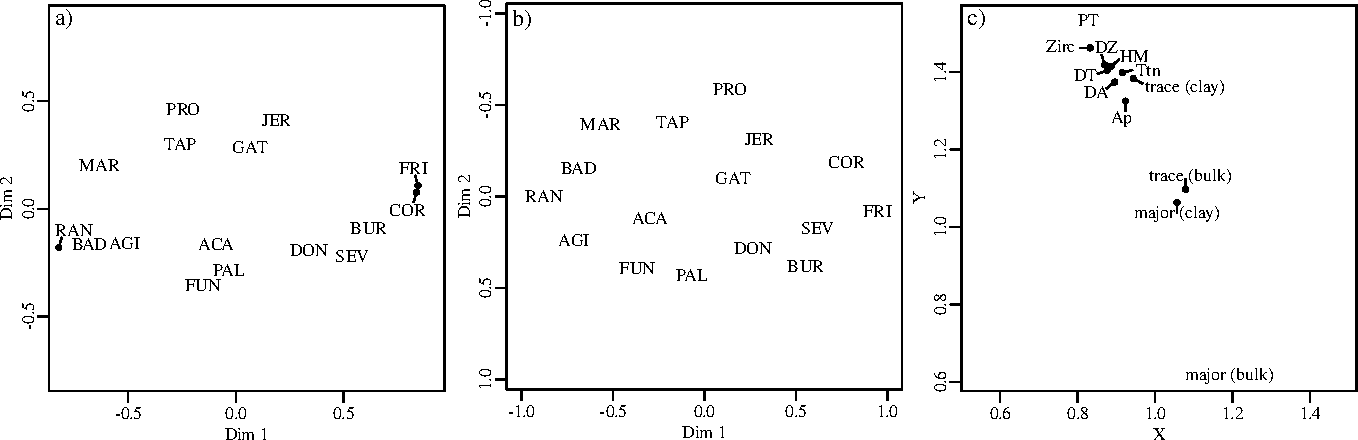
\includegraphics[height=.7\textheight]{Fig5.pdf}
\caption{a) Procrustes analysis and b) group configuration of a 3-way
  MDS analysis of the 12 provenance proxies from the SNSM, using
  method 1; c) the source weights of the 3-way MDS analysis. DA, DT
  and DZ stand for U-Pb age distributions of detrital apatite,
  titanite and zircon, respectively; Ap, Ttn and Zirc for the varietal
  apatite, titanite and zircon data; PT and HM for petrography and
  heavy minerals; and major and trace for the chemical composition of
  the bulk sediment and clay fractions. Note that the vertical axis of
  panel b) has been flipped to facilitate comparison with panel a).}
\label{fig:multimethod}
\end{figure}

\section{Implementation in \texttt{provenance}}\label{sec:R}

All the algorithms described in this paper have been implemented in a
free and open \texttt{R} package called \texttt{provenance}
\cite{vermeesch2016a}. \texttt{provenance} comes with a query-based
user interface that does not require any knowledge of \texttt{R}.  The
following paragraphs, however, will focus on the command line
interface.  Version~4.1 of the package adds a new \texttt{varietal}
data class, which can be populated from a \texttt{.csv} input file
using the \texttt{read.varietal} function:

\begin{verbatim}
library(provenance)
Ttn <- read.varietal(fname="Ttn_chem.csv",snames=3)
\end{verbatim}

\noindent where \verb|Ttn_chem.csv| is a compositional data table
containing the concatenated compositions of all the samples. The
column names of this table specify its components, whereas the row
names consist of an alphanumeric prefix corresponding to the sample
name, followed by a unique identifier for each analysis. The
\texttt{sname} argument either specifies a vector of prefixes, or the
length of the prefix. The output of the \texttt{read.varietal}
function consists of a list containing the input table, a vector of
sample names (in this case the prefixes extracted from the row names),
the name of the dataset, and the dissimilarity measure (\texttt{KS}
for Kolmogorov-Smirnov by default). The varietal data object can be
passed on to several other functions of the \texttt{provenance}
package. To subject the varietal data to (2-way) MDS using method~1
(treatment-by-row):
\begin{verbatim}
plot(MDS(Ttn,method="KS"))
\end{verbatim}

\noindent where the output of the \texttt{MDS} function is nested as
input in the overloaded \texttt{plot} function. To analyse the
titanite chemistry data by method~2 (treatment-by-column), using
Procrustes analysis:
\begin{verbatim}
plot(procrustes(Ttn))
\end{verbatim}

\noindent and using 3-way MDS \cite[a.k.a. `Individual Differences
  Scaling' or INDSCAL]{carroll1970}:
\begin{verbatim}
plot(indscal(Ttn))
\end{verbatim}

Method~3 requires linear programming, which is currently delegated to
either the \texttt{transport} or \texttt{approxOT} package
\cite{schumacher2022, dunipace2021}. Using the former:
\begin{verbatim}
plot(MDS(Ttn,method="W2",package="transport"))
\end{verbatim}

To combine multiple provenance proxies by Procrustes analysis, for
example using titanite, apatite and zircon chemistry (using method~3);
titanite, apatite and zircon U-Pb ages; heavy minerals and
petrography; and the major and trace element compositions of the bulk
sediment and clay fractions:
\begin{verbatim}
Ttn <- read.varietal(fname="Ttn_chem.csv",snames=3,method="KS")
Ap <- read.varietal(fname="Ap_chem.csv",snames=3,method="KS")
Zr <- read.varietal(fname="Zr_chem.csv",snames=3,method="KS")
DA <- read.distributional("DA.csv")
DT <- read.distributional("DT.csv")
DZ <- read.distributional("DZ.csv")
HM <- read.counts("HM.csv")
PT <- read.counts("PT.csv")
major_bulk <- read.compositional("Major_BULK.csv")
major_clay <- read.compositional("Major_CLAY.csv")
trace_bulk <- read.compositional("Trace_BULK.csv")
trace_clay <- read.compositional("Trace_CLAY.csv")
proc <- procrustes(Ttn,Ap,Zr,DA,DT,DZ,HM,PT,
                   major_bulk,major_clay,trace_bulk,trace_clay)
plot(proc)
\end{verbatim}

Note that the dissimilarity measure (i.e., $W_2$) is added to the data
by the \texttt{read.varietal} function, unlike the earlier example,
which used the default KS method. Analysing the same holistic dataset
by 3-way MDS:
\begin{verbatim}
plot(indscal(Ttn,Ap,Zr,DA,DT,DZ,HM,PT,
             major_bulk,major_clay,trace_bulk,trace_clay))
\end{verbatim}

\section{Conclusions}\label{sec:conclusions}

This paper introduced three different approaches to quantify the
dissimilarity between different samples in varietal datasets.  These
approaches can be used to populate dissimilarity matrices, which can
be analysed by MDS.\medskip

Methods~1, 2 and 3 produce reassuringly similar results for the
titanite chemistry data of the SNSM.  This suggests that even though
the three methods each consider different parts of the dataset, they
all retain the key inter-sample similarities and
differences. Comparable results are obtained for the other provenance
proxies, which confirms that varietal data do carry a robust and
reproducible provenance signature. The consistency of the results
obtained from a single dataset with the combined dataset of all the
provenance proxies further lends credence to the conclusions drawn
from the multivariate ordination analyses.\medskip

In principle, method~3 is the most powerful of the three approaches,
because it directly converts varietal data to dissimilarity matrices
and jointly considers all the compositional information that is stored
in the varietal data. In contrast, methods~1 and 2 require the
conversion of the varietal data to distributional data. Some
information is lost in this additional step. For method~1, only the
information contained in the first principal component is retained.
For method~2, the connection between the various columns of the
compositional data members of the varietal data structure is lost,
including any constant sum constraint.\medskip

Despite these limitations, methods~1 and 2 also offer some advantages
over method~3. Whereas the connection between the MDS configuration
and the compositional data variables is lost in the process of
calculating the Wasserstein-2 distance, this connection is partially
retained in method~1, and nearly completely in method~2. Thus, the
results of methods~1 and 2 are easier to verify and interpret than
those of method~3.\medskip

For example, in the case of the titanite chemistry data from the SNSM,
samples MAR and COR plot on opposite sides of the MDS configuration
(Figure~\ref{fig:method3}), and it is not immediately clear which
compositional variables cause these differences. However, inspection
of PC1 in method~1 (Figure~\ref{fig:method1}.a) or, more directly, the
subject weights in method~2 (Figure~\ref{fig:method2}.c) reveals that
these trends reflect differences in the W-Al-Pb-Fe vs. actinides and
light rare earth abundances.\medskip

At first glance, the Procrustes analysis (Figure~\ref{fig:method2}.a)
does not seem to offer any advantage over 3-way MDS. However, it is
useful to repeat the caveat that was previously raised by
\citeA{borg2005}, which is that the source weights of a 3-way MDS
analysis are sensitive to noise and are not as stable as the user
might wish. Thus it is important not to over-interpret the results of
3-way MDS.\medskip

Inspection of Figures~\ref{fig:method3}.b and c also suggests that the
$W_2$ distance is more sensitive to small sample fluctuations than the
KS-distance. This is clearest for samples PRO and JER, which contain
only 15 and 20 titanite analyses, respectively. Although the $W_2$
results are, on average, more precise than the corresponding $KS$
results, the difference in precision between small and large samples
is greater for the $W_2$-distance than the $KS$-distance. This
explains the distant location of PRO and JER on the MDS configuration
of Figure~\ref{fig:method3}.a.\medskip

The limitations of method-3 become less important when it is used to
combine varietal data with other provenance proxies
(Section~\ref{sec:3way}). The full SNSM dataset contains no fewer than
126,408 measurements, spanning 12 dimensions worth of information.  It
is impossible to capture the full richness of datasets like this in a
few simple scatterplots such as Figure~\ref{fig:multimethod}. However,
the internal consistency of the SNSM results, and their sensible
geological interpretation, suggest that the approaches described in
this paper are capable of separating geologically meaningful signals
from noise. Further applications will be needed to confirm if this
applies in other geological settings as well.

\section*{Open Research Section}
All the data and software introduced in this paper is publicly
available on the Comprehensive R Archive Network (CRAN,
https://CRAN.R-project.org/package=provenance) and on GitHub
(\url{https://github.com/pvermees/provenance/},
doi:10.5281/zenodo.7633857). The raw data files can be found at
\url{https://github.com/pvermees/provenance/tree/master/inst/SNSM/}

\section*{Acknowledgments} This work was supported by NERC Standard Grant
\#NE/T001518/1, awarded to PV, and by project CA 2099/2-1 of the
Deutsche Forschungsgemeinschaft (DFG), awarded to LC. AGL is funded by
a Junior Research Fellowship from Merton College, Oxford. DC is
supported in part by a research grant from Science Foundation Ireland
(SFI) under Grant Number 13/RC/2092\_P2 (iCRAG, the SFI Research
Centre in Applied Geosciences). We would like to thank Glenn
R. Sharman and an anonymous reviewer for positive and constructive
feedback.

\begin{thebibliography}{}

\bibitem [\protect \citeauthoryear {%
Aitchison%
}{%
Aitchison%
}{%
{\protect \APACyear {1983}}%
}]{%
aitchison1983}
\APACinsertmetastar {%
aitchison1983}%
\begin{APACrefauthors}%
Aitchison, J.%
\end{APACrefauthors}%
\unskip\
\newblock
\APACrefYearMonthDay{1983}{}{}.
\newblock
{\BBOQ}\APACrefatitle {Principal component analysis of compositional data}
  {Principal component analysis of compositional data}.{\BBCQ}
\newblock
\APACjournalVolNumPages{Biometrika}{70}{1}{57-65}.
\newblock
\begin{APACrefDOI} \doi{10.1093/biomet/70.1.57} \end{APACrefDOI}
\PrintBackRefs{\CurrentBib}

\bibitem [\protect \citeauthoryear {%
Aitchison%
}{%
Aitchison%
}{%
{\protect \APACyear {1986}}%
}]{%
aitchison1986}
\APACinsertmetastar {%
aitchison1986}%
\begin{APACrefauthors}%
Aitchison, J.%
\end{APACrefauthors}%
\unskip\
\newblock
\APACrefYear{1986}.
\newblock
\APACrefbtitle {The statistical analysis of compositional data} {The
  statistical analysis of compositional data}.
\newblock
\APACaddressPublisher{}{London, Chapman and Hall}.
\PrintBackRefs{\CurrentBib}

\bibitem [\protect \citeauthoryear {%
Arabie%
, Carroll%
\BCBL {}\ \BBA {} DeSarbo%
}{%
Arabie%
\ \protect \BOthers {.}}{%
{\protect \APACyear {1987}}%
}]{%
arabie1987}
\APACinsertmetastar {%
arabie1987}%
\begin{APACrefauthors}%
Arabie, P.%
, Carroll, J\BPBI D.%
\BCBL {}\ \BBA {} DeSarbo, W\BPBI S.%
\end{APACrefauthors}%
\unskip\
\newblock
\APACrefYear{1987}.
\newblock
\APACrefbtitle {Three Way Scaling: A Guide to Multidimensional Scaling and
  Clustering} {Three way scaling: A guide to multidimensional scaling and
  clustering}\ (\BVOL~65).
\newblock
\APACaddressPublisher{}{Sage}.
\PrintBackRefs{\CurrentBib}

\bibitem [\protect \citeauthoryear {%
Borg%
\ \BBA {} Groenen%
}{%
Borg%
\ \BBA {} Groenen%
}{%
{\protect \APACyear {2005}}%
}]{%
borg2005}
\APACinsertmetastar {%
borg2005}%
\begin{APACrefauthors}%
Borg, I.%
\BCBT {}\ \BBA {} Groenen, P\BPBI J.%
\end{APACrefauthors}%
\unskip\
\newblock
\APACrefYear{2005}.
\newblock
\APACrefbtitle {Modern multidimensional scaling: Theory and applications}
  {Modern multidimensional scaling: Theory and applications}.
\newblock
\APACaddressPublisher{}{Springer}.
\PrintBackRefs{\CurrentBib}

\bibitem [\protect \citeauthoryear {%
Caracciolo%
\ \protect \BOthers {.}}{%
Caracciolo%
\ \protect \BOthers {.}}{%
{\protect \APACyear {in review}}%
}]{%
caracciolo2023}
\APACinsertmetastar {%
caracciolo2023}%
\begin{APACrefauthors}%
Caracciolo, L.%
, Hatzenb\"{u}hler, D.%
, Chew, D.%
, Weltje, G\BPBI J.%
, Vermeesch, P.%
, Piraquive, A.%
\BDBL {}Villanueva, N.%
\end{APACrefauthors}%
\unskip\
\newblock
\APACrefYearMonthDay{in review}{}{}.
\newblock
{\BBOQ}\APACrefatitle {What do we measure in Provenance Analysis? A
  controversial case study on Sediment Generation in the Sierra Nevada de Santa
  Marta (Colombia)} {What do we measure in provenance analysis? a controversial
  case study on sediment generation in the sierra nevada de santa marta
  (colombia)}.{\BBCQ}
\newblock
\APACjournalVolNumPages{Geological Society of Americal Bulletin}{}{}{}.
\PrintBackRefs{\CurrentBib}

\bibitem [\protect \citeauthoryear {%
Carroll%
\ \BBA {} Chang%
}{%
Carroll%
\ \BBA {} Chang%
}{%
{\protect \APACyear {1970}}%
}]{%
carroll1970}
\APACinsertmetastar {%
carroll1970}%
\begin{APACrefauthors}%
Carroll, J\BPBI D.%
\BCBT {}\ \BBA {} Chang, J\BHBI J.%
\end{APACrefauthors}%
\unskip\
\newblock
\APACrefYearMonthDay{1970}{}{}.
\newblock
{\BBOQ}\APACrefatitle {{Analysis of individual differences in multidimensional
  scaling via an N-way generalization of `Eckart-Young' decomposition}}
  {{Analysis of individual differences in multidimensional scaling via an N-way
  generalization of `Eckart-Young' decomposition}}.{\BBCQ}
\newblock
\APACjournalVolNumPages{Psychometrika}{35}{3}{283--319}.
\PrintBackRefs{\CurrentBib}

\bibitem [\protect \citeauthoryear {%
Dunipace%
}{%
Dunipace%
}{%
{\protect \APACyear {2021}}%
}]{%
dunipace2021}
\APACinsertmetastar {%
dunipace2021}%
\begin{APACrefauthors}%
Dunipace, E\BPBI A.%
\end{APACrefauthors}%
\unskip\
\newblock
\APACrefYearMonthDay{2021}{}{}.
\newblock
{\BBOQ}\APACrefatitle {{approxOT}: approximate optimal transport} {{approxOT}:
  approximate optimal transport}{\BBCQ}\ [\bibcomputersoftwaremanual].
\newblock
\begin{APACrefURL} \url{https://github.com/ericdunipace/approxOT}
  \end{APACrefURL}
\newblock
\APACrefnote{R package version 0.1}
\PrintBackRefs{\CurrentBib}

\bibitem [\protect \citeauthoryear {%
Gower%
}{%
Gower%
}{%
{\protect \APACyear {1975}}%
}]{%
gower1975}
\APACinsertmetastar {%
gower1975}%
\begin{APACrefauthors}%
Gower, J\BPBI C.%
\end{APACrefauthors}%
\unskip\
\newblock
\APACrefYearMonthDay{1975}{}{}.
\newblock
{\BBOQ}\APACrefatitle {Generalized procrustes analysis} {Generalized procrustes
  analysis}.{\BBCQ}
\newblock
\APACjournalVolNumPages{Psychometrika}{40}{1}{33--51}.
\PrintBackRefs{\CurrentBib}

\bibitem [\protect \citeauthoryear {%
Greenacre%
}{%
Greenacre%
}{%
{\protect \APACyear {1984}}%
}]{%
greenacre1984}
\APACinsertmetastar {%
greenacre1984}%
\begin{APACrefauthors}%
Greenacre, M\BPBI J.%
\end{APACrefauthors}%
\unskip\
\newblock
\APACrefYear{1984}.
\newblock
\APACrefbtitle {Theory and applications of correspondence analysis} {Theory and
  applications of correspondence analysis}.
\newblock
\APACaddressPublisher{}{Academic Press}.
\PrintBackRefs{\CurrentBib}

\bibitem [\protect \citeauthoryear {%
Kruskal%
\ \BBA {} Wish%
}{%
Kruskal%
\ \BBA {} Wish%
}{%
{\protect \APACyear {1978}}%
}]{%
kruskal1978}
\APACinsertmetastar {%
kruskal1978}%
\begin{APACrefauthors}%
Kruskal, J\BPBI B.%
\BCBT {}\ \BBA {} Wish, M.%
\end{APACrefauthors}%
\unskip\
\newblock
\APACrefYear{1978}.
\newblock
\APACrefbtitle {Multidimensional scaling} {Multidimensional scaling}\ (\BVOL\
  07-011).
\newblock
\APACaddressPublisher{}{Sage Publications, Beverly Hills and London}.
\PrintBackRefs{\CurrentBib}

\bibitem [\protect \citeauthoryear {%
Lipp%
\ \BBA {} Vermeesch%
}{%
Lipp%
\ \BBA {} Vermeesch%
}{%
{\protect \APACyear {2022}}%
}]{%
lipp2022}
\APACinsertmetastar {%
lipp2022}%
\begin{APACrefauthors}%
Lipp, A\BPBI G.%
\BCBT {}\ \BBA {} Vermeesch, P.%
\end{APACrefauthors}%
\unskip\
\newblock
\APACrefYearMonthDay{2022}{}{}.
\newblock
{\BBOQ}\APACrefatitle {{Comparing detrital age spectra, and other geological
  distributions, using the Wasserstein distance}} {{Comparing detrital age
  spectra, and other geological distributions, using the Wasserstein
  distance}}.{\BBCQ}
\newblock
\APACjournalVolNumPages{Earth and Planetary Science Letters}{}{}{}.
\newblock
\begin{APACrefDOI} \doi{10.31223/X5TM02} \end{APACrefDOI}
\PrintBackRefs{\CurrentBib}

\bibitem [\protect \citeauthoryear {%
Morton%
}{%
Morton%
}{%
{\protect \APACyear {1985}}%
}]{%
morton1985b}
\APACinsertmetastar {%
morton1985b}%
\begin{APACrefauthors}%
Morton, A\BPBI C.%
\end{APACrefauthors}%
\unskip\
\newblock
\APACrefYearMonthDay{1985}{}{}.
\newblock
{\BBOQ}\APACrefatitle {Heavy minerals in provenance studies} {Heavy minerals in
  provenance studies}.{\BBCQ}
\newblock
\BIn{} \APACrefbtitle {Provenance of arenites} {Provenance of arenites}\
  (\BPGS\ 249--277).
\newblock
\APACaddressPublisher{}{Springer}.
\PrintBackRefs{\CurrentBib}

\bibitem [\protect \citeauthoryear {%
Morton%
}{%
Morton%
}{%
{\protect \APACyear {1991}}%
}]{%
morton1991}
\APACinsertmetastar {%
morton1991}%
\begin{APACrefauthors}%
Morton, A\BPBI C.%
\end{APACrefauthors}%
\unskip\
\newblock
\APACrefYearMonthDay{1991}{}{}.
\newblock
{\BBOQ}\APACrefatitle {Geochemical studies of detrital heavy minerals and their
  application to provenance research} {Geochemical studies of detrital heavy
  minerals and their application to provenance research}.{\BBCQ}
\newblock
\BIn{} A.~Morton, S.~Todd\BCBL {}\ \BBA {} P\BPBI D\BPBI W.~Haughton\ (\BEDS),
  \APACrefbtitle {{Developments in Sedimentary Provenance Studies}}
  {{Developments in Sedimentary Provenance Studies}}\ (\BVOL~57, \BPGS\
  31--45).
\newblock
\APACaddressPublisher{}{Geological Society of London}.
\PrintBackRefs{\CurrentBib}

\bibitem [\protect \citeauthoryear {%
Schuhmacher%
\ \protect \BOthers {.}}{%
Schuhmacher%
\ \protect \BOthers {.}}{%
{\protect \APACyear {2022}}%
}]{%
schumacher2022}
\APACinsertmetastar {%
schumacher2022}%
\begin{APACrefauthors}%
Schuhmacher, D.%
, B\"{a}hre, B.%
, Gottschlich, C.%
, Hartmann, V.%
, Heinemann, F.%
\BCBL {}\ \BBA {} Schmitzer, B.%
\end{APACrefauthors}%
\unskip\
\newblock
\APACrefYearMonthDay{2022}{}{}.
\newblock
{\BBOQ}\APACrefatitle {{transport}: Computation of Optimal Transport Plans and
  Wasserstein Distances} {{transport}: Computation of optimal transport plans
  and wasserstein distances}{\BBCQ}\ [\bibcomputersoftwaremanual].
\newblock
\begin{APACrefURL} \url{https://cran.r-project.org/package=transport}
  \end{APACrefURL}
\newblock
\APACrefnote{R package version 0.12-4}
\PrintBackRefs{\CurrentBib}

\bibitem [\protect \citeauthoryear {%
Shepard%
}{%
Shepard%
}{%
{\protect \APACyear {1980}}%
}]{%
shepard1980}
\APACinsertmetastar {%
shepard1980}%
\begin{APACrefauthors}%
Shepard, R\BPBI N.%
\end{APACrefauthors}%
\unskip\
\newblock
\APACrefYearMonthDay{1980}{}{}.
\newblock
{\BBOQ}\APACrefatitle {Multidimensional scaling, tree-fitting, and clustering}
  {Multidimensional scaling, tree-fitting, and clustering}.{\BBCQ}
\newblock
\APACjournalVolNumPages{Science}{210}{4468}{390--398}.
\PrintBackRefs{\CurrentBib}

\bibitem [\protect \citeauthoryear {%
Vermeesch%
}{%
Vermeesch%
}{%
{\protect \APACyear {2013}}%
}]{%
vermeesch2013}
\APACinsertmetastar {%
vermeesch2013}%
\begin{APACrefauthors}%
Vermeesch, P.%
\end{APACrefauthors}%
\unskip\
\newblock
\APACrefYearMonthDay{2013}{}{}.
\newblock
{\BBOQ}\APACrefatitle {Multi-sample comparison of detrital age distributions}
  {Multi-sample comparison of detrital age distributions}.{\BBCQ}
\newblock
\APACjournalVolNumPages{Chemical Geology}{341}{}{140--146}.
\PrintBackRefs{\CurrentBib}

\bibitem [\protect \citeauthoryear {%
Vermeesch%
}{%
Vermeesch%
}{%
{\protect \APACyear {2018}}%
{\protect \APACexlab {{\protect \BCnt {1}}}}}]{%
vermeesch2018b}
\APACinsertmetastar {%
vermeesch2018b}%
\begin{APACrefauthors}%
Vermeesch, P.%
\end{APACrefauthors}%
\unskip\
\newblock
\APACrefYearMonthDay{2018{\protect \BCnt {1}}}{}{}.
\newblock
{\BBOQ}\APACrefatitle {{Dissimilarity measures in detrital geochronology}}
  {{Dissimilarity measures in detrital geochronology}}.{\BBCQ}
\newblock
\APACjournalVolNumPages{Earth-Science Reviews}{178}{}{310-321}.
\newblock
\begin{APACrefDOI} \doi{10.1016/j.earscirev.2017.11.027} \end{APACrefDOI}
\PrintBackRefs{\CurrentBib}

\bibitem [\protect \citeauthoryear {%
Vermeesch%
}{%
Vermeesch%
}{%
{\protect \APACyear {2018}}%
{\protect \APACexlab {{\protect \BCnt {2}}}}}]{%
vermeesch2018d}
\APACinsertmetastar {%
vermeesch2018d}%
\begin{APACrefauthors}%
Vermeesch, P.%
\end{APACrefauthors}%
\unskip\
\newblock
\APACrefYearMonthDay{2018{\protect \BCnt {2}}}{}{}.
\newblock
{\BBOQ}\APACrefatitle {Statistical models for point-counting data} {Statistical
  models for point-counting data}.{\BBCQ}
\newblock
\APACjournalVolNumPages{Earth and Planetary Science Letters}{501}{}{1--7}.
\PrintBackRefs{\CurrentBib}

\bibitem [\protect \citeauthoryear {%
Vermeesch%
}{%
Vermeesch%
}{%
{\protect \APACyear {2019}}%
}]{%
vermeesch2019a}
\APACinsertmetastar {%
vermeesch2019a}%
\begin{APACrefauthors}%
Vermeesch, P.%
\end{APACrefauthors}%
\unskip\
\newblock
\APACrefYearMonthDay{2019}{}{}.
\newblock
{\BBOQ}\APACrefatitle {{Exploratory Analysis of Provenance Data Using R and the
  Provenance Package}} {{Exploratory Analysis of Provenance Data Using R and
  the Provenance Package}}.{\BBCQ}
\newblock
\APACjournalVolNumPages{Minerals}{9}{3}{193}.
\PrintBackRefs{\CurrentBib}

\bibitem [\protect \citeauthoryear {%
Vermeesch%
\ \BBA {} Garzanti%
}{%
Vermeesch%
\ \BBA {} Garzanti%
}{%
{\protect \APACyear {2015}}%
}]{%
vermeesch2015}
\APACinsertmetastar {%
vermeesch2015}%
\begin{APACrefauthors}%
Vermeesch, P.%
\BCBT {}\ \BBA {} Garzanti, E.%
\end{APACrefauthors}%
\unskip\
\newblock
\APACrefYearMonthDay{2015}{}{}.
\newblock
{\BBOQ}\APACrefatitle {{Making geological sense of `Big Data' in sedimentary
  provenance analysis}} {{Making geological sense of `Big Data' in sedimentary
  provenance analysis}}.{\BBCQ}
\newblock
\APACjournalVolNumPages{Chemical Geology}{409}{}{20--27}.
\PrintBackRefs{\CurrentBib}

\bibitem [\protect \citeauthoryear {%
Vermeesch%
, Resentini%
\BCBL {}\ \BBA {} Garzanti%
}{%
Vermeesch%
\ \protect \BOthers {.}}{%
{\protect \APACyear {2016}}%
}]{%
vermeesch2016a}
\APACinsertmetastar {%
vermeesch2016a}%
\begin{APACrefauthors}%
Vermeesch, P.%
, Resentini, A.%
\BCBL {}\ \BBA {} Garzanti, E.%
\end{APACrefauthors}%
\unskip\
\newblock
\APACrefYearMonthDay{2016}{}{}.
\newblock
{\BBOQ}\APACrefatitle {{An R package for statistical provenance analysis}} {{An
  R package for statistical provenance analysis}}.{\BBCQ}
\newblock
\APACjournalVolNumPages{Sedimentary Geology}{}{}{}.
\PrintBackRefs{\CurrentBib}

\bibitem [\protect \citeauthoryear {%
Villani%
}{%
Villani%
}{%
{\protect \APACyear {2021}}%
}]{%
villani2021}
\APACinsertmetastar {%
villani2021}%
\begin{APACrefauthors}%
Villani, C.%
\end{APACrefauthors}%
\unskip\
\newblock
\APACrefYear{2021}.
\newblock
\APACrefbtitle {Topics in optimal transportation} {Topics in optimal
  transportation}\ (\BVOL~58).
\newblock
\APACaddressPublisher{}{American Mathematical Soc.}
\PrintBackRefs{\CurrentBib}

\end{thebibliography}

\end{document}
